    %?%%%%%%%%%%%%%%%%%%%%%%%%%%%%% HIPOTEZY %%%%%%%%%%%%%%%%%%%%%%%%%%%%%%
    \subsection{Hipotezy}
    Głównym celem badania było sprawdzenie, czy kolor okularów wpływa na czas skupienia na żółtej torbie (TFD-Y bag).
    W ramach tego celu sformułowano następujące hipotezy:
    \begin{itemize}
        \item $H_0$: Średnie czasy skupienia na żółtej torbie (TFD-Y bag) są równe dla wszystkich grup kolorów okularów.
        \item $H_1$: Nie dla wszystkich grup kolorów okularów średnie czasy skupienia na żółtej torbie (TFD-Y bag) są równe.
    \end{itemize}
    
    Dodatkowo, w ramach badania, sprawdzono wpływ doświadczenia na czas skupienia na żółtej torbie (TFD-Y bag).
    W tym celu sformułowano następujące hipotezy:
    \begin{itemize}
        \item $H_0$: Nie ma różnicy w czasie skupienia na żółtej torbie (TFD-Y bag) pomiędzy grupami z doświadczeniem i bez doświadczenia.
        \item $H_1$: Grupa z doświadczaniem ma dłuższy czas skupienia na żółtej torbie (TFD-Y bag) niż grupa bez doświadczenia.
    \end{itemize}
    
    %?%%%%%%%%%%%%%%%%%%%%%%%%%%%%% Analiza deskryptywna %%%%%%%%%%%%%%%%%%%%%%%%%%%%%%
    \subsection{Analiza deskryptywna zmiennej}
    \begin{table}[H]
        \centering
        \caption{Opis deskryptywny zmiennej TFD dla obiektu żółta torba (yellow bag).}
        \begin{tabular}{|c|c|c|c|}%
            \hline
            \bfseries Miara & \bfseries Gogle przezroczyste & \bfseries Gogle czerwone & \bfseries Gogle żółte% specify table head
            \csvreader[head to column names]{./../res_tables/summaryTFD_yBag.csv}{}% use head of csv as column names
            {\\\hline\Miara & \num{\T} & \num{\R} & \num{\Y}}% specify your columns here
            \\\hline    
        \end{tabular}
        \label{tab:summaryTFD_yBag}
    \end{table}
    \begin{figure}[H]
        \centering
        \resizebox{0.7 \columnwidth}{!}{%
        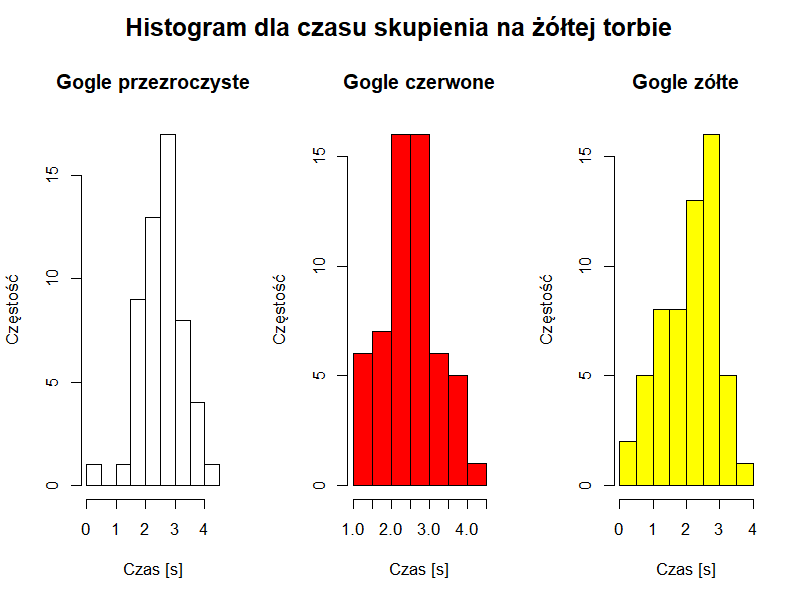
\includegraphics{./../res_plots/Histogram_dla_czasu_skupienia_na_żółtej_torbie.png}%
        }
        \label{fig:histTFD_yBag}
        \caption{Histogram dla zmiennej TFD dla obiektu żółta torba (yellow bag).}
    \end{figure}
    \begin{figure}[H]
        \centering
        \resizebox{0.7 \columnwidth}{!}{%
        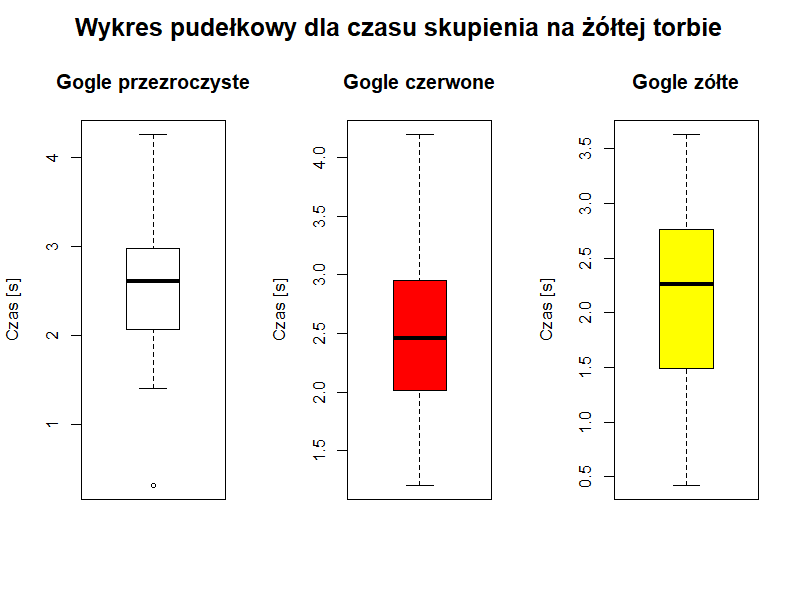
\includegraphics{./../res_plots/Wykres_pudełkowy_dla_czasu_skupienia_na_żółtej_torbie.png}%
        }
        \label{fig:boxTFD_yBag}
        \caption{Wykres pudełkowy dla zmiennej TFD dla obiektu żółta torba (yellow bag).}
    \end{figure}

    %?%%%%%%%%%%%%%%%%%%%%%%%%%%%%% Analiza deskryptywna %%%%%%%%%%%%%%%%%%%%%%%%%%%%%%
    \subsection{Równoliczność grup}
    Dla sprawdzenia równoliczności grup wykonano test $\chi^2$ z następującymi hipotezami:
    \begin{itemize}
        \item $H_0$: liczebności grup są równe.
        \item $H_1$: liczebności grup są różne.
    \end{itemize}
    Otrzymana wartość wynosi \textbf{$p=0.926$}, co oznacza, że na poziomie istotności $\alpha=0.05$
    nie ma podstaw do odrzucenia hipotezy zerowej. Na tej podstawie można stwierdzić, że \textbf{liczebności grup są równe}.
    
    %?%%%%%%%%%%%%%%%%%%%%%%%%%%%%% NORMALNOŚĆ %%%%%%%%%%%%%%%%%%%%%%%%%%%%%%

    \subsection{Normalność zmiennej w grupach}
    Do analizy normalności rozkładu zastosowane zostały histogramy oraz test Shapiro-Wilka. Oprócz analizy standardowych wartości
    zmiennej TFD-Y bag, przeprowadzono również analizy dla ich przekształceń: pierwiastka z X, pierwiastka kwadratowego z X oraz logarytmu z X.

    \begin{table}[H]
        \centering
        \caption{Wyniki testu Shapiro-Wilka dla czasu skupienia na żółtej torbie (bez przekształceń).}
        \begin{tabular}{|c|c|c|}%
            \hline
            \bfseries Kolor okularów & \bfseries Wartość p & \bfseries Czy rozkład normalny% specify table head
            \csvreader[head to column names]{./../res_tables/yBag_shapiro_default.csv}{}% use head of csv as column names
            {\\\hline\kolorGogli & \num{\shapiroP} & \czyNormalny}% specify your columns here
            \\\hline    
        \end{tabular}
        \label{tab:shapiroYBagDefault}
    \end{table}
    \begin{figure}[H]
        \centering
        \resizebox{0.7 \columnwidth}{!}{%
        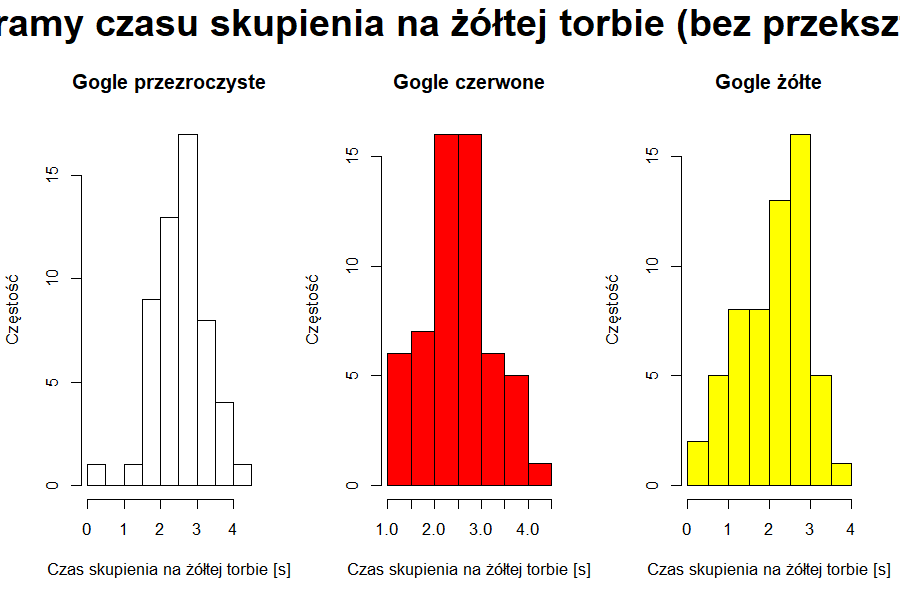
\includegraphics{./../res_plots/historgram_dla_TFD_yBag_default.png}%
        }
        \caption{Histogram dla czasu skupienia na żółtej torbie (bez przekształceń).}
        \label{fig:histYBagDefault}
    \end{figure}

    \begin{table}[H]
        \centering
        \caption{Wyniki testu Shapiro-Wilka dla czasu skupienia na żółtej torbie (pierwiastek z X).}
        \begin{tabular}{|c|c|c|}%
            \hline
            \bfseries Kolor okularów & \bfseries Wartość p & \bfseries Czy rozkład normalny% specify table head
            \csvreader[head to column names]{./../res_tables/yBag_shapiro_x^0.5.csv}{}% use head of csv as column names
            {\\\hline\kolorGogli & \num{\shapiroP} & \czyNormalny}% specify your columns here
            \\\hline    
        \end{tabular}
        \label{tab:shapiroYBagPow0.5}
    \end{table}
    \begin{figure}[H]
        \centering
        \resizebox{0.7 \columnwidth}{!}{%
        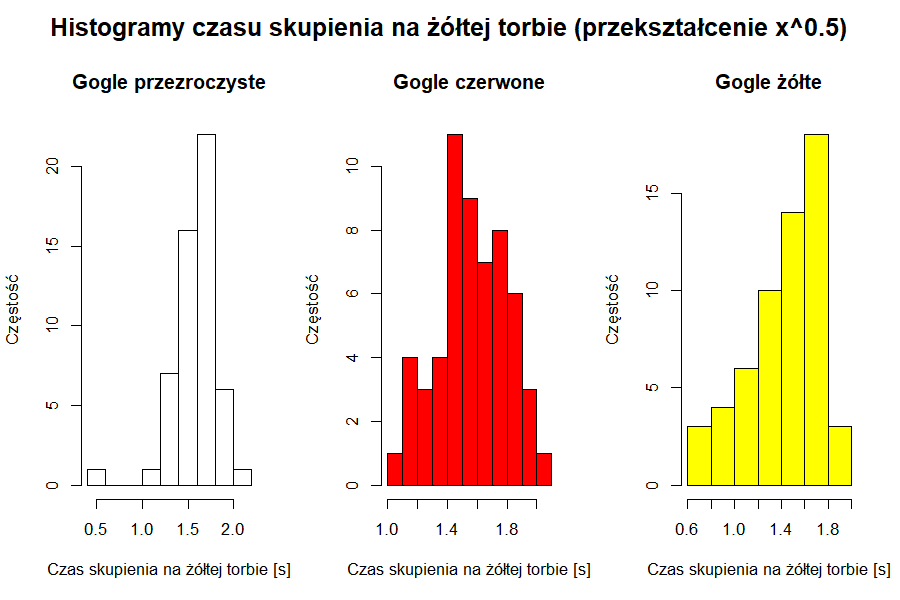
\includegraphics{./../res_plots/historgram_dla_TFD_yBag_x^0.5.png}%
        }
        \caption{Histogram dla czasu skupienia na żółtej torbie (pierwiastek z X).}
        \label{fig:histYBagPow0.5}
    \end{figure}

    \begin{table}[H]
        \centering
        \caption{Wyniki testu Shapiro-Wilka dla czasu skupienia na żółtej torbie (pierwiastek kwadratowy z X).}
        \begin{tabular}{|c|c|c|}%
            \hline
            \bfseries Kolor okularów & \bfseries Wartość p & \bfseries Czy rozkład normalny% specify table head
            \csvreader[head to column names]{./../res_tables/yBag_shapiro_x^0.25.csv}{}% use head of csv as column names
            {\\\hline\kolorGogli & \num{\shapiroP} & \czyNormalny}% specify your columns here
            \\\hline    
        \end{tabular}
        \label{tab:shapiroYBagPow0.25}
    \end{table}
    \begin{figure}[H]
        \centering
        \resizebox{0.7 \columnwidth}{!}{%
        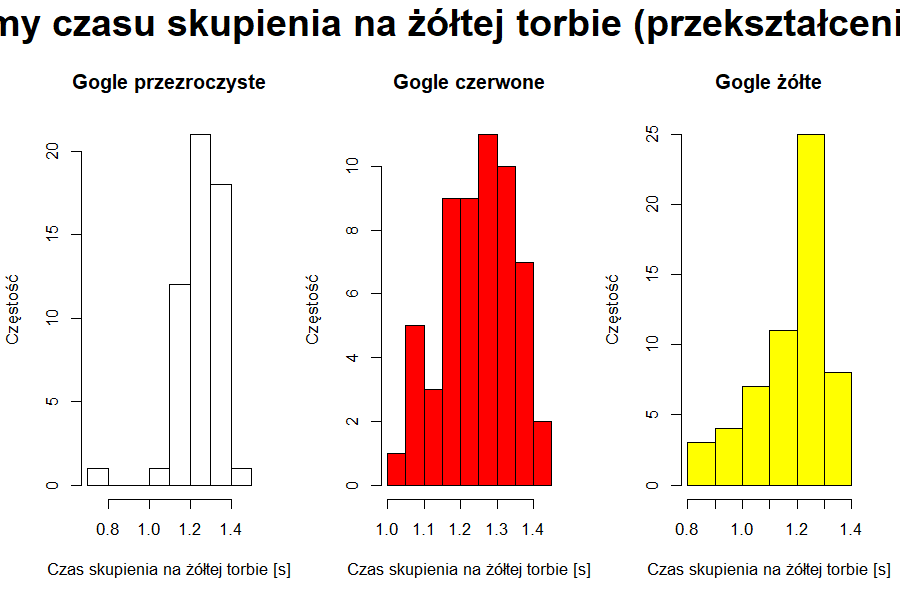
\includegraphics{./../res_plots/historgram_dla_TFD_yBag_x^0.25.png}%
        }
        \caption{Histogram dla czasu skupienia na żółtej torbie (pierwiastek kwadratowy z X).}
        \label{fig:histYBagPow0.25}
    \end{figure}

    \begin{table}[H]
        \centering
        \caption{Wyniki testu Shapiro-Wilka dla czasu skupienia na żółtej torbie (logarytm z X).}
        \begin{tabular}{|c|c|c|}%
            \hline
            \bfseries Kolor okularów & \bfseries Wartość p & \bfseries Czy rozkład normalny% specify table head
            \csvreader[head to column names]{./../res_tables/yBag_shapiro_log(x).csv}{}% use head of csv as column names
            {\\\hline\kolorGogli & \num{\shapiroP} & \czyNormalny}% specify your columns here
            \\\hline    
        \end{tabular}
        \label{tab:shapiroYBagLog}
    \end{table}
    \begin{figure}[H]
        \centering
        \resizebox{0.7 \columnwidth}{!}{%
        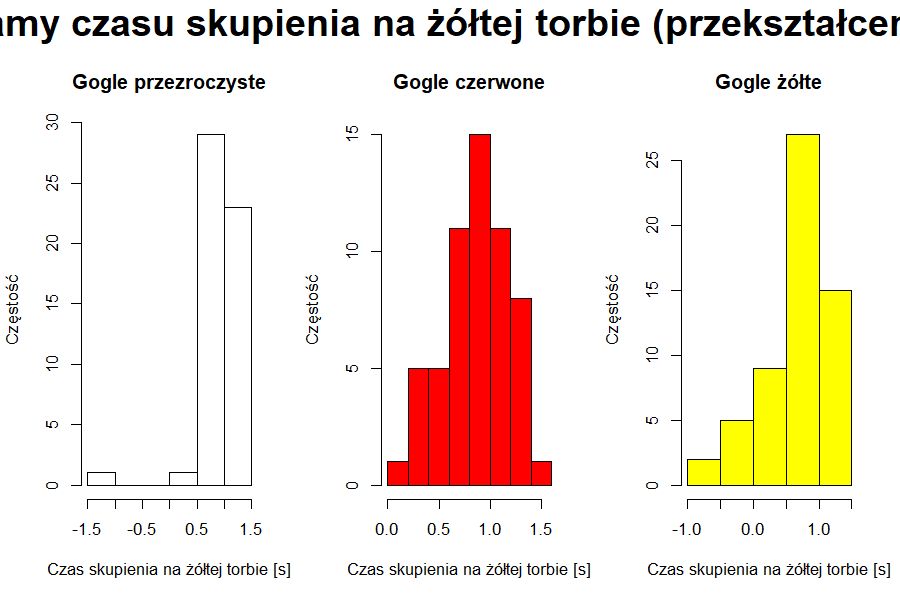
\includegraphics{./../res_plots/historgram_dla_TFD_yBag_log(x).png}%
        }
        \caption{Histogram dla czasu skupienia na żółtej torbie (logarytm z X).}
        \label{fig:histYBagLog}
    \end{figure}
   
    \begin{figure}[H]
        \centering
        \resizebox{0.7 \columnwidth}{!}{%
        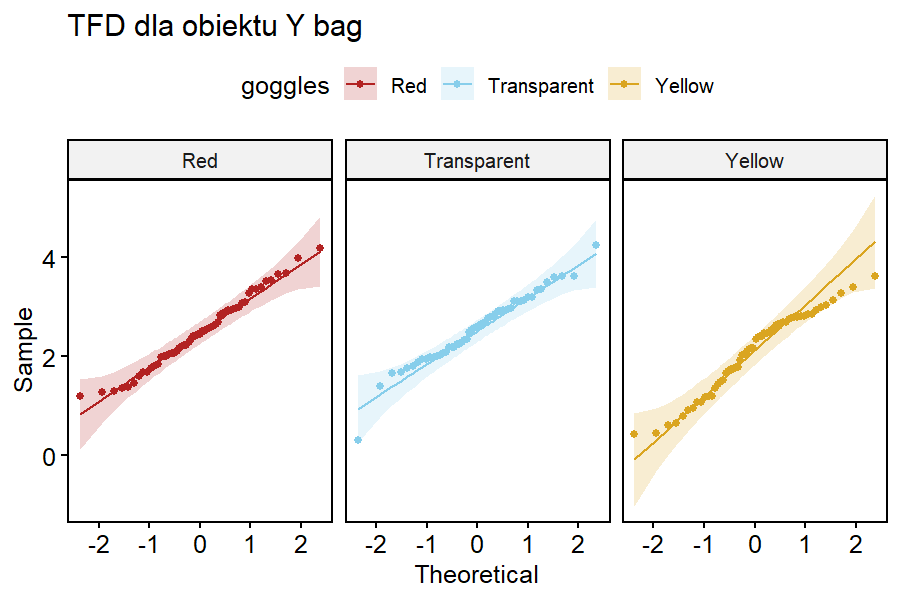
\includegraphics{./../res_plots/qqplot_dla_TFD_yBag.png}%
        }
        \caption{Wykres kwartyl-kwartyl dla czasu skupienia na żółtej torbie }
        \label{fig:qqplotYBag}
    \end{figure}
     
    Na podstawie otrzymanych histogramów [\ref{fig:histYBagDefault} - \ref{fig:histYBagLog}] i wyników testu Shapiro-Wilka 
    [\ref{tab:shapiroYBagDefault} - \ref{tab:shapiroYBagLog}] można stwierdzić, że \textbf{rozkłady są  najbliższe normalności dla danych bez przekształceń}.
    Dla grupy czerwonej i przezroczystej wykonane testy wskazują na normalność rozkładu zmiennej TFD-Y bag.
    Dla grupy żółtej testy shapiro-wilka [\ref{tab:shapiroYBagDefault}] nie pozwala na przyjcie H0 świadczącej o normalności rozkładu,
    niemniej otrzymana wartość p jest bliska granicy istotności $\alpha=0.05$ oraz wykresy histogramu [\ref{fig:histYBagDefault}] i wykresy
    kwartyl-kwartyl [\ref{fig:qqplotYBag}] sugerują, że rozkład jest zbliżony do normalnego.
    Dlatego można przyjąć, że \textbf{rozkład zmiennej TFD-Y bag jest normalny we wszystkich grupach}. 

    \subsection{Równość wariancji w grupach}
        Na podstawie wyników z sekcji \textit{''Normalność zmiennej w grupach''} stwierdzono, 
        normalność rozkładu zmiennej TFD-Y bag w grupach. Mając jednak na uwadze, że rozkład
        zmiennej TFD-Y bag w grupie żółtej nie jest idealnie normalny, przeprowadzono test Levene'a
        wycentrowanego na podstawie średniej, który jest bardziej odporny na odchylenia od normalności.

        Hipotezy:
        \begin{itemize}
            \item $H_0$: wariancje we wszystkich grupach są równe.
            \item $H_1$:  co najmniej jedna grupa ma inną wariancję.
        \end{itemize}
        Otrzymana wartość wynosi $p=0.240$, co oznacza, że na poziomie istotności $\alpha=0.05$
        nie ma podstaw do odrzucenia hipotezy zerowej. Na tej podstawie można stwierdzić, że \textbf{wariancje są równe}.

    \subsection{Równość średnich w grupach} %TODO
        \subsubsection{Uzasadnienie wyboru testu na podstawie wyników analiz z punktów 2-5} %TODO
        \subsubsection{Przeprowadzenie testu - wynik i wnioski} %TODO
    \subsection{Wpływ doświadczenia na zmienną TFD} %TODO